
Several CT scans have been run to search for a corrosion layer. Additionally, another scan has been run using thermal neutrons to compare both results. The result is shown for the EXRADIN and PTW chambers in Figure \ref{fig:Reconstruction-of-PTW-EXRADIN}.

\begin{figure}[!h]
\centering
\begin{minipage}{0.45\textwidth}
    \centering
    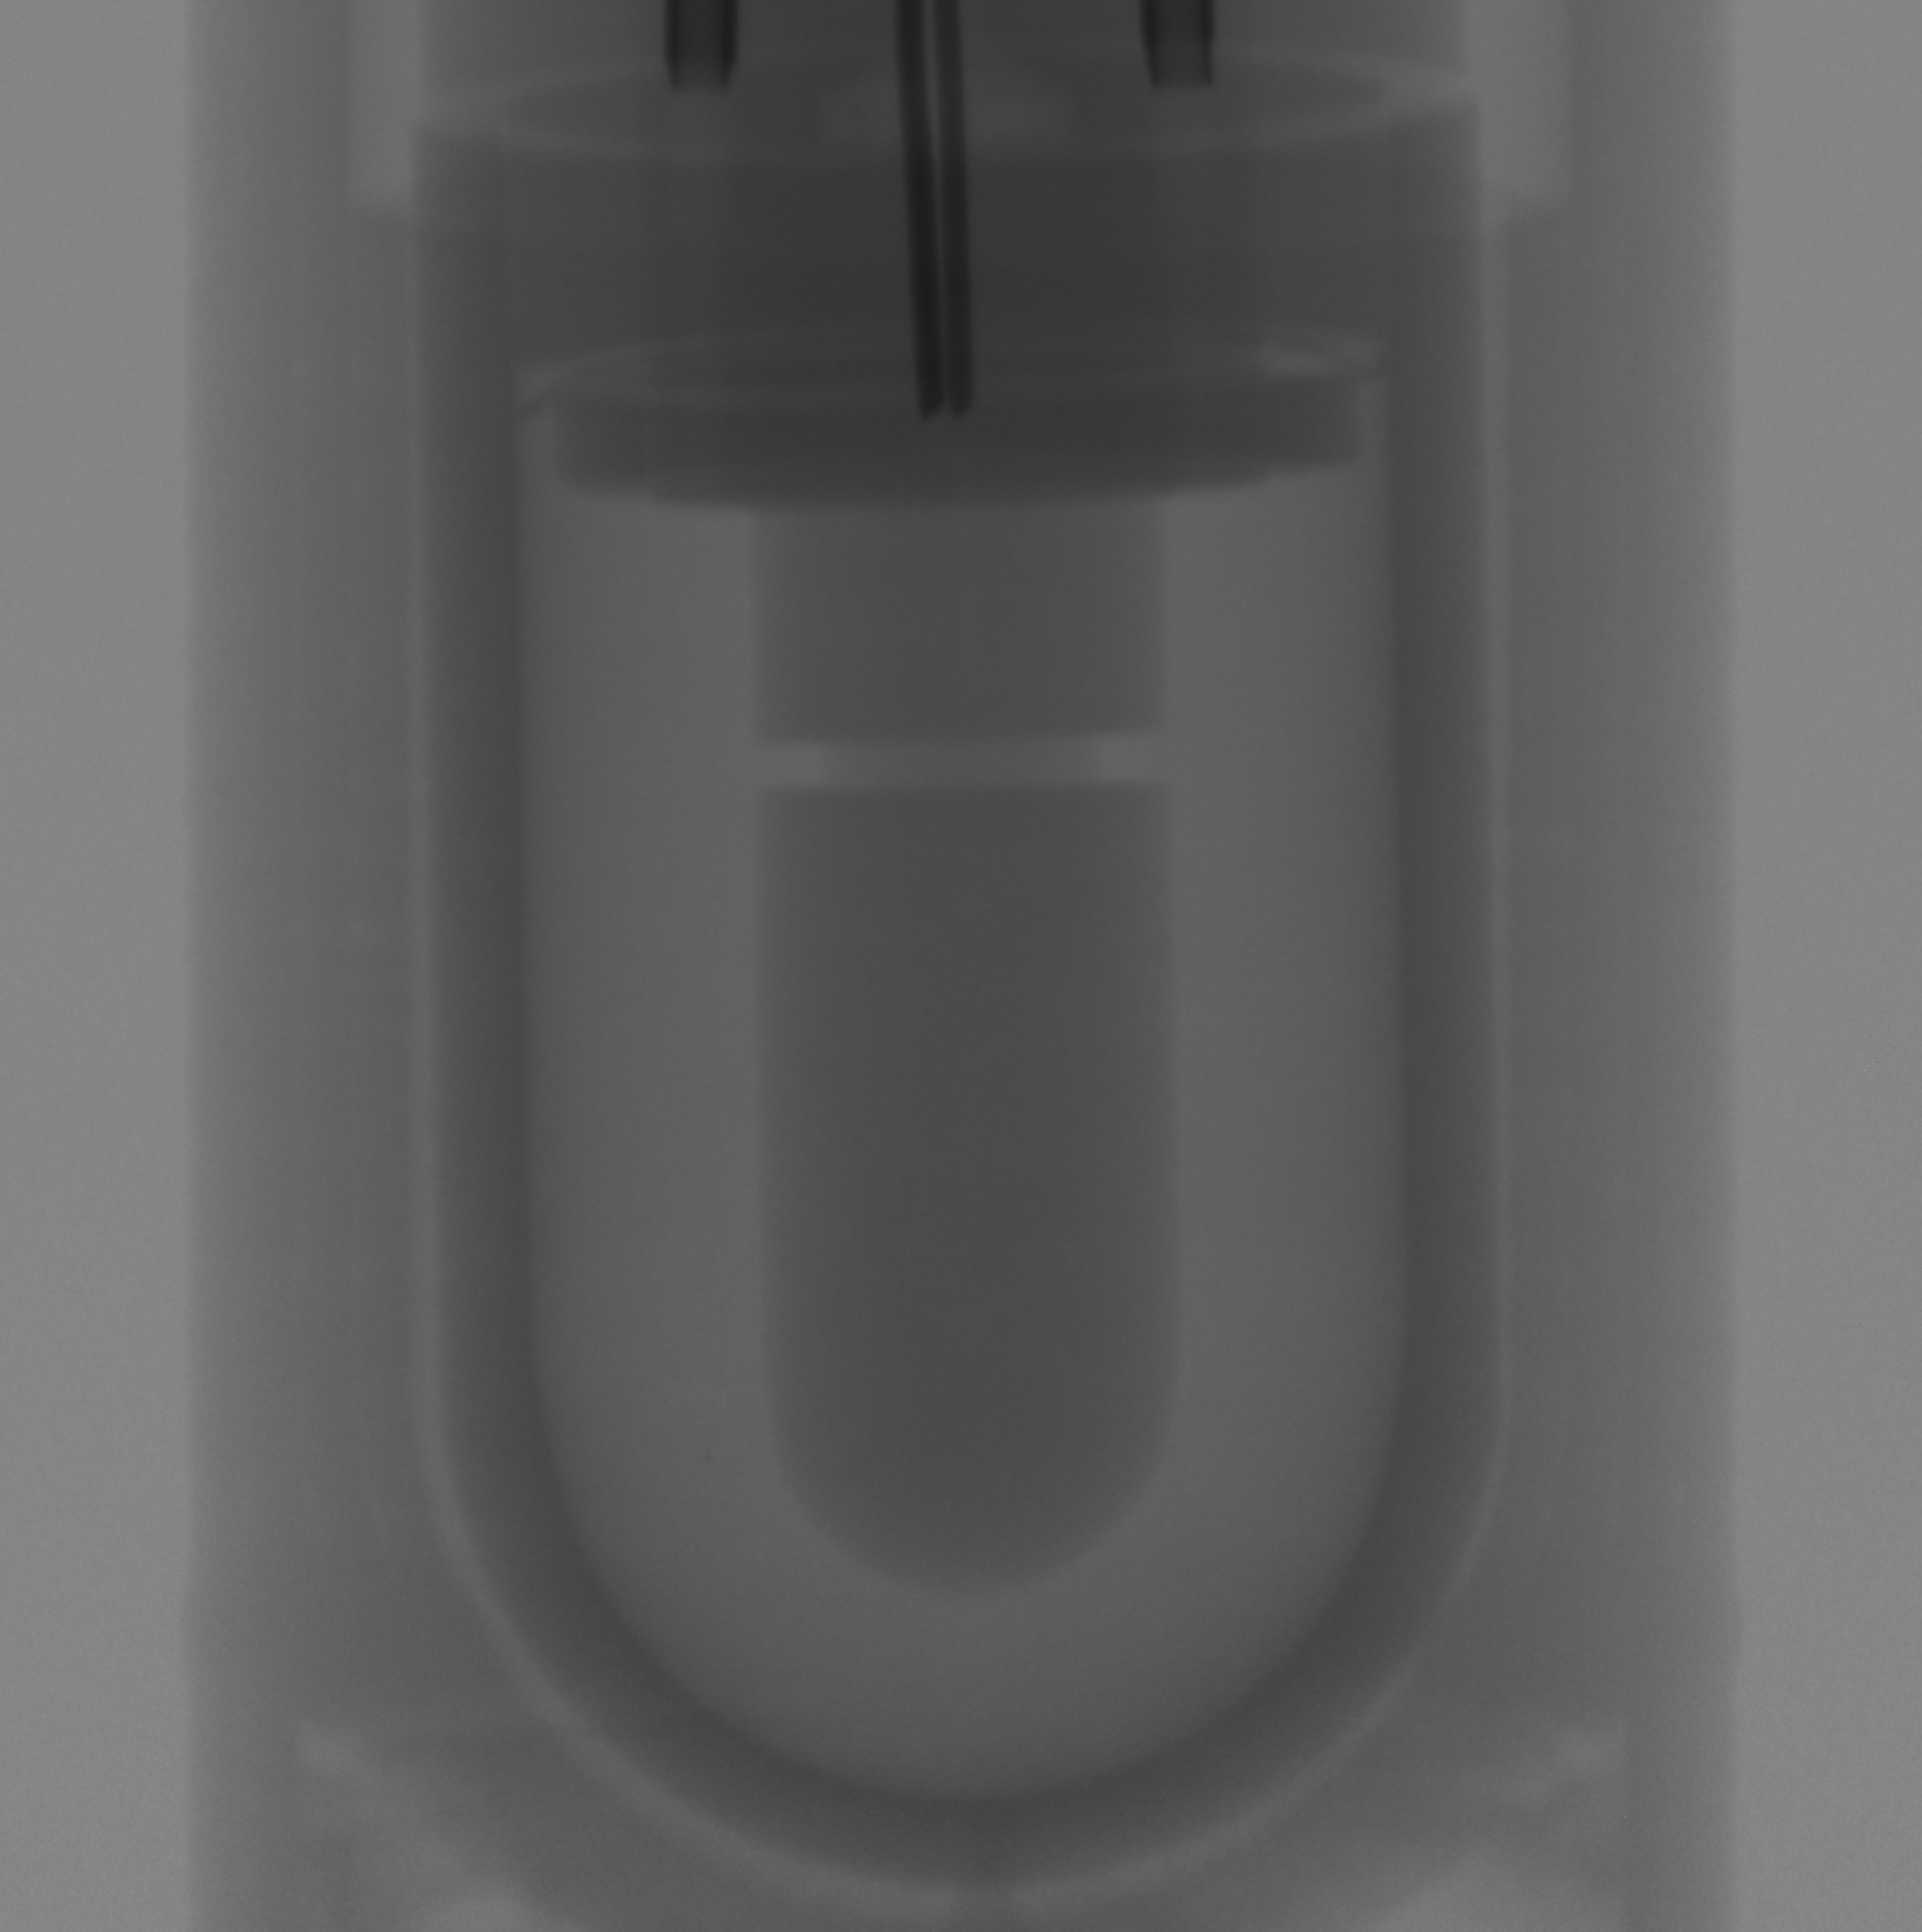
\includegraphics[width=0.9\linewidth]{Master Thesis Manuel Galdon/figures/Imaging/reconstruction of EXRADIN CT corrosion Mg.png}
    %\caption{3D reconstruction of the EXRADIN chamber}
    %\label{fig:EXRADIN-CT}
\end{minipage}
\hfill
\begin{minipage}{0.45\textwidth}
    \centering
    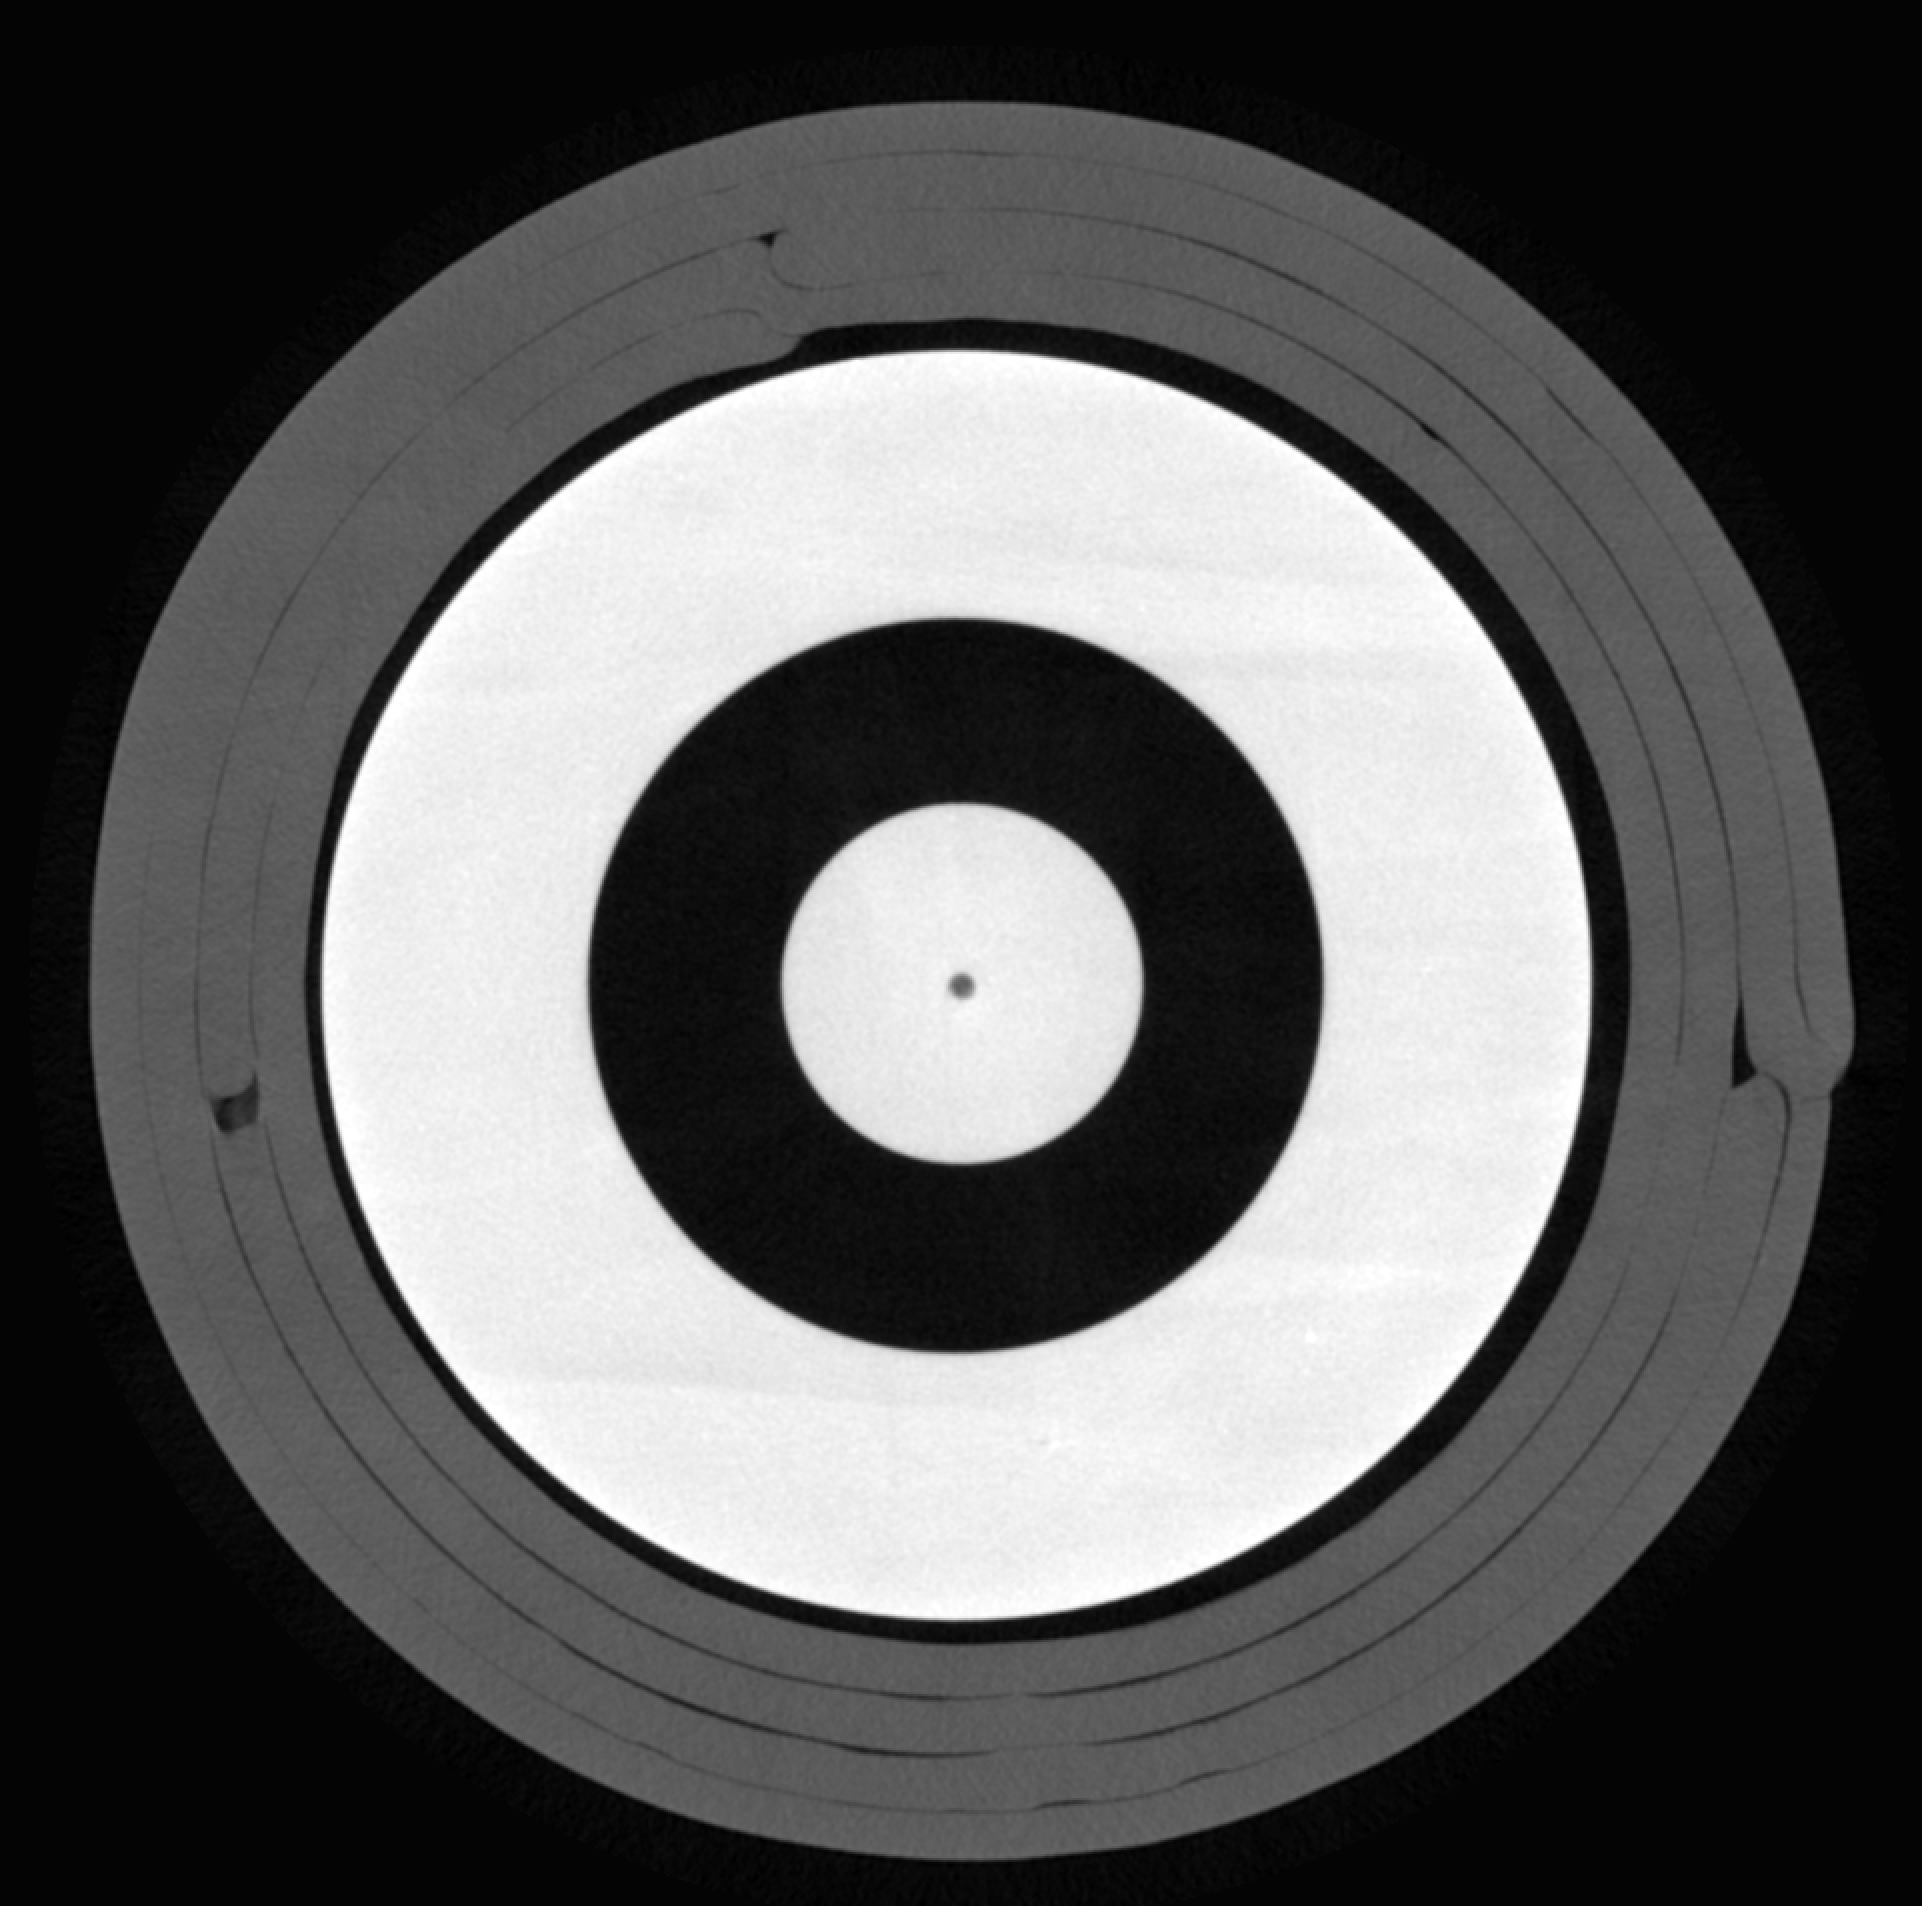
\includegraphics[width=0.9\linewidth]{Master Thesis Manuel Galdon/figures/Imaging/PTW CT corrosion Mg_1.png}
    %\caption{Image of the PTW chamber}
    %\label{fig:PTW-CT}
\end{minipage}
\caption{X-ray CT scan of EXRADIN chamber (left) and the PTW TM33054 chamber (right). Both devices are made of magnesium.}
\label{fig:Reconstruction-of-PTW-EXRADIN}
\end{figure}

The inner structure is shown in both images. There are several flaws in the material that can be seen on the scan. There are small air bubbles in the center of the chamber as of the black color that represents the air.


As illustrated in the next image, small bubbles are also allocated within the magnesium structure (the white region):
\clearpage
\begin{figure}[!h]
    \centering
    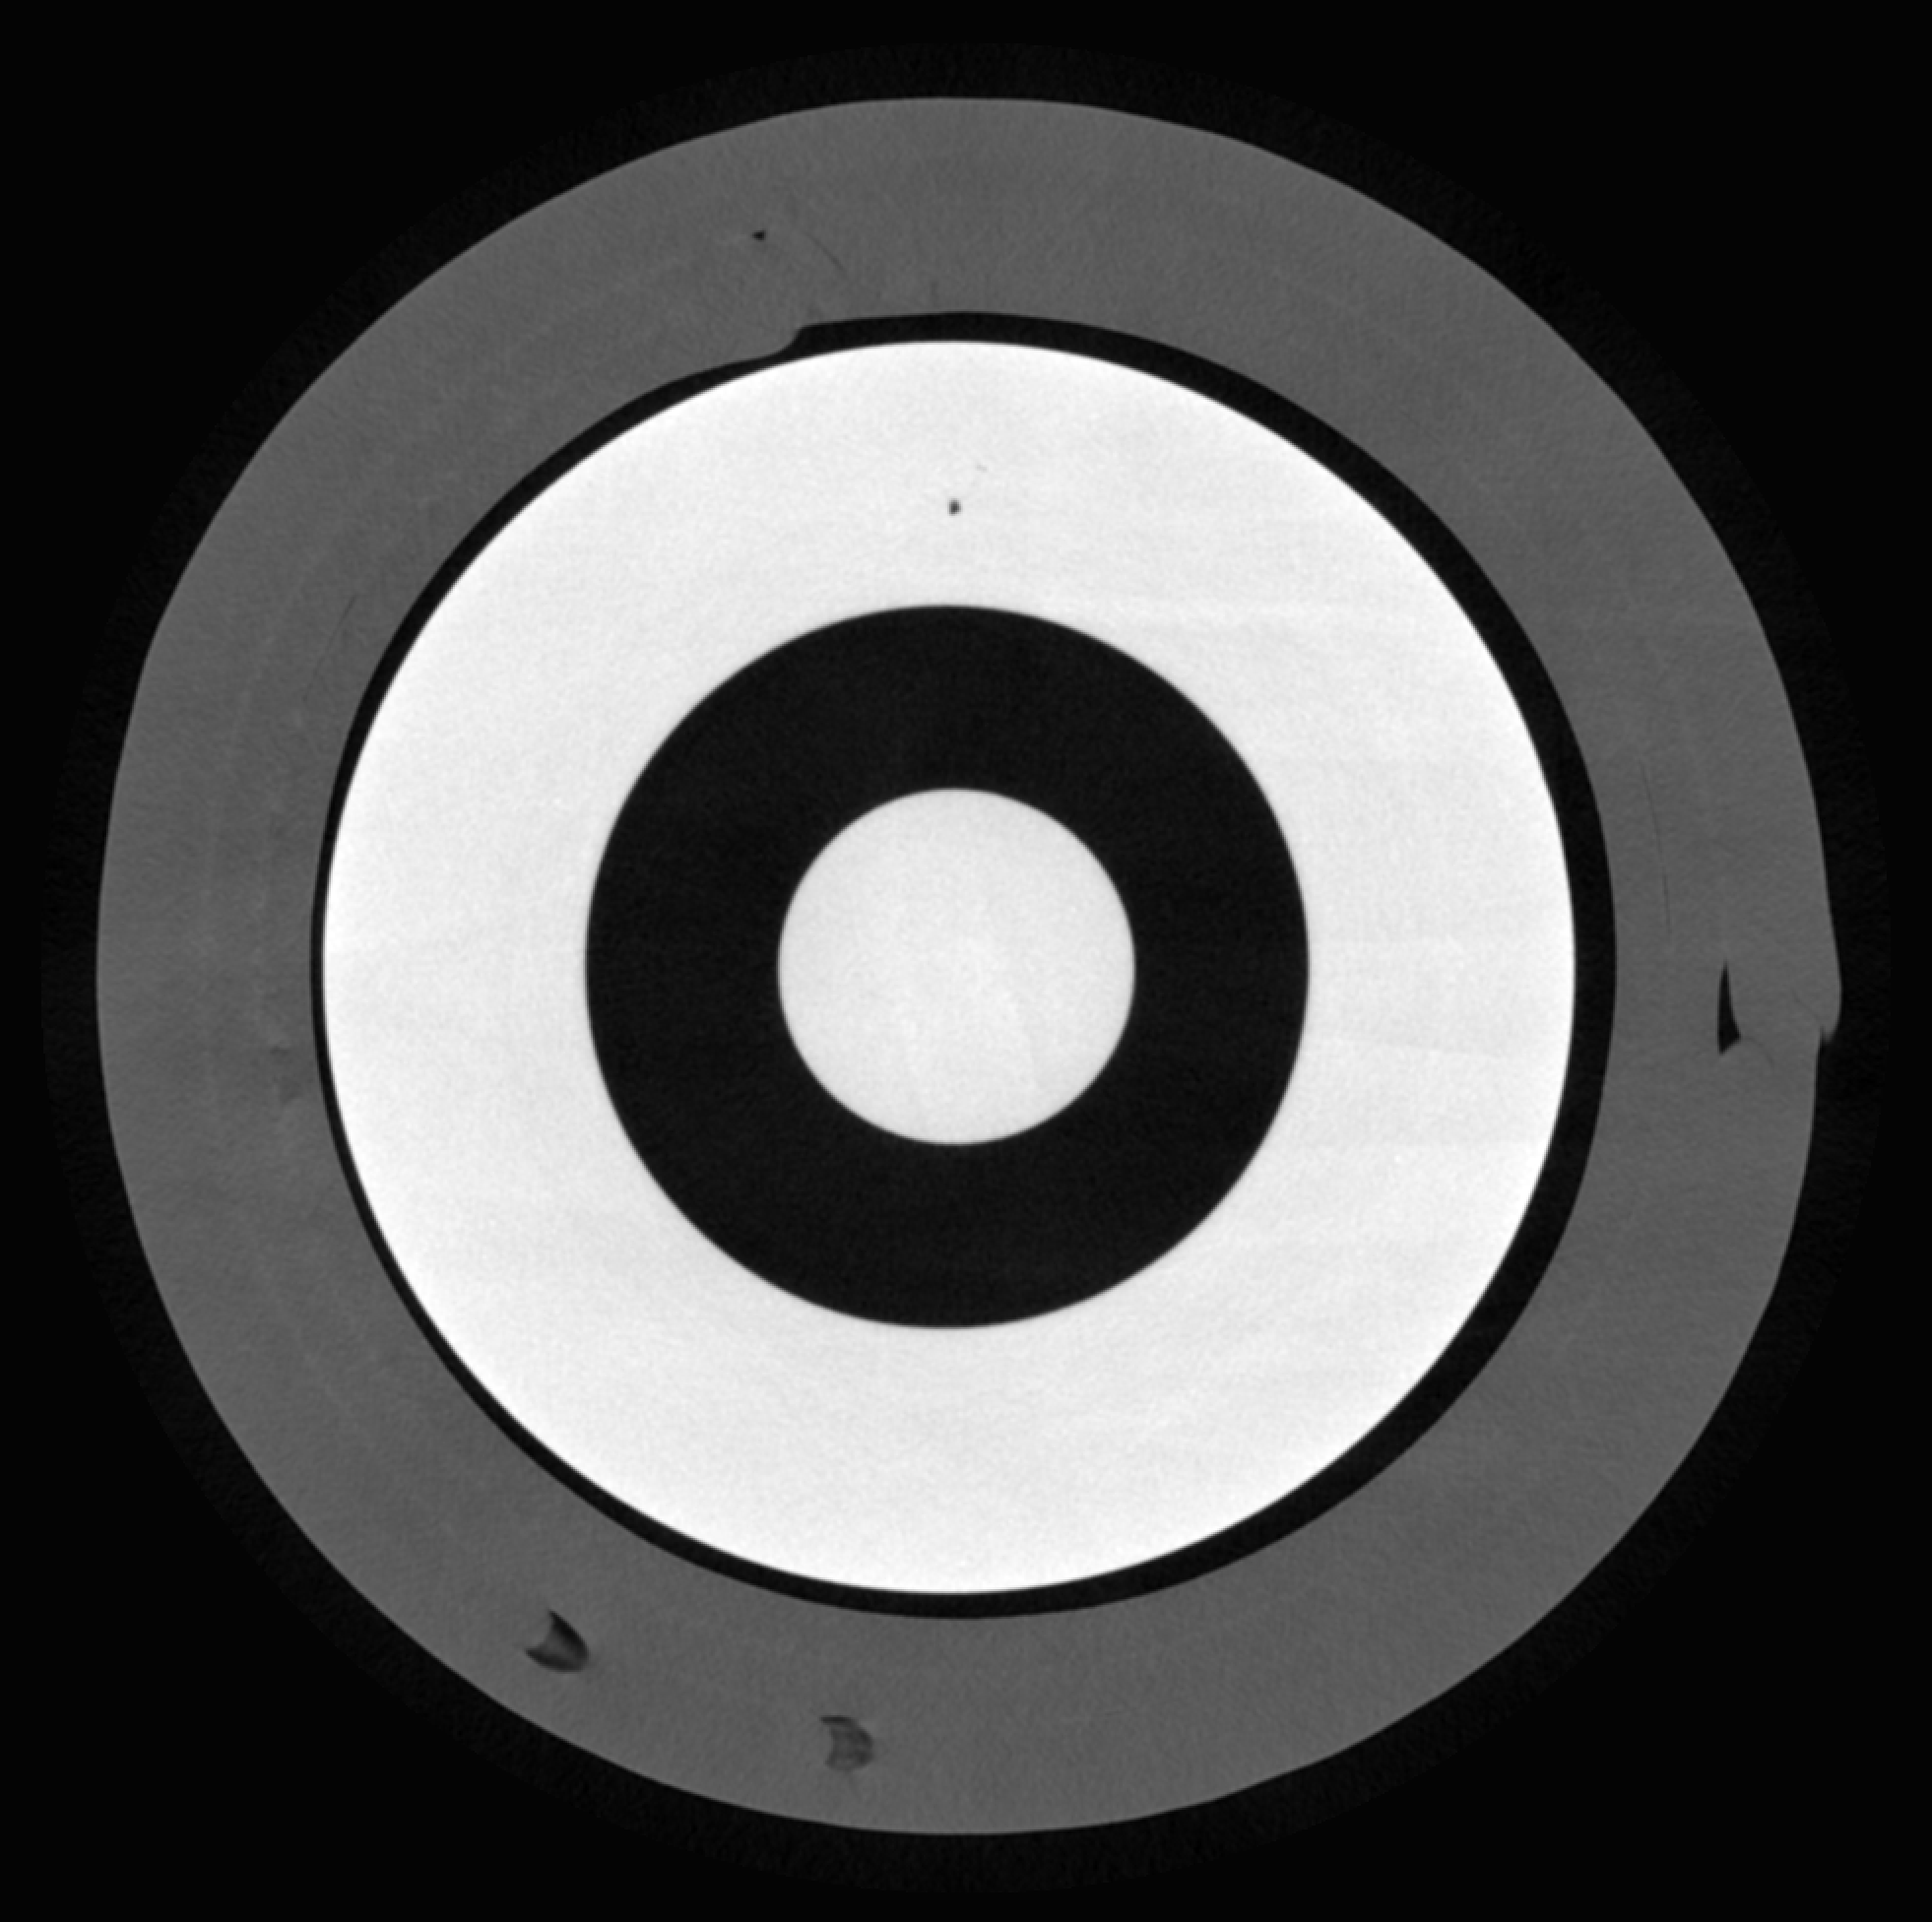
\includegraphics[scale = 0.2]{Master Thesis Manuel Galdon/figures/Imaging/PTW CT corrosion Mg_2.png}
    \caption{Image of the X-ray CT scan of the PTW TM33054 ionization chamber.}
    \label{fig:Image of PTW CT scan}
\end{figure}

The same imperfections in the materials appear in the successive images taken along the axial direction of the chamber. However, there are no evidences of corrosion over the surfaces in any of the images. This fact can be attributed to the null interaction of the corrosion with photons. 

Since neutrons interact differently with the chamber, the outcome of the neutron scan reveals that the surface of the magnesium wall is covered with a different composite. In Figure \ref{fig:Neutron scan vs plot}, the neutron scan of the PTW TM33054 magnesium chamber is represented along with a plot of the gray values against the width of the chamber. The distances of the plot have been scaled to the actual size of the chamber.


\begin{figure}[!h]
\centering
\begin{minipage}{0.45\textwidth}
    \centering
    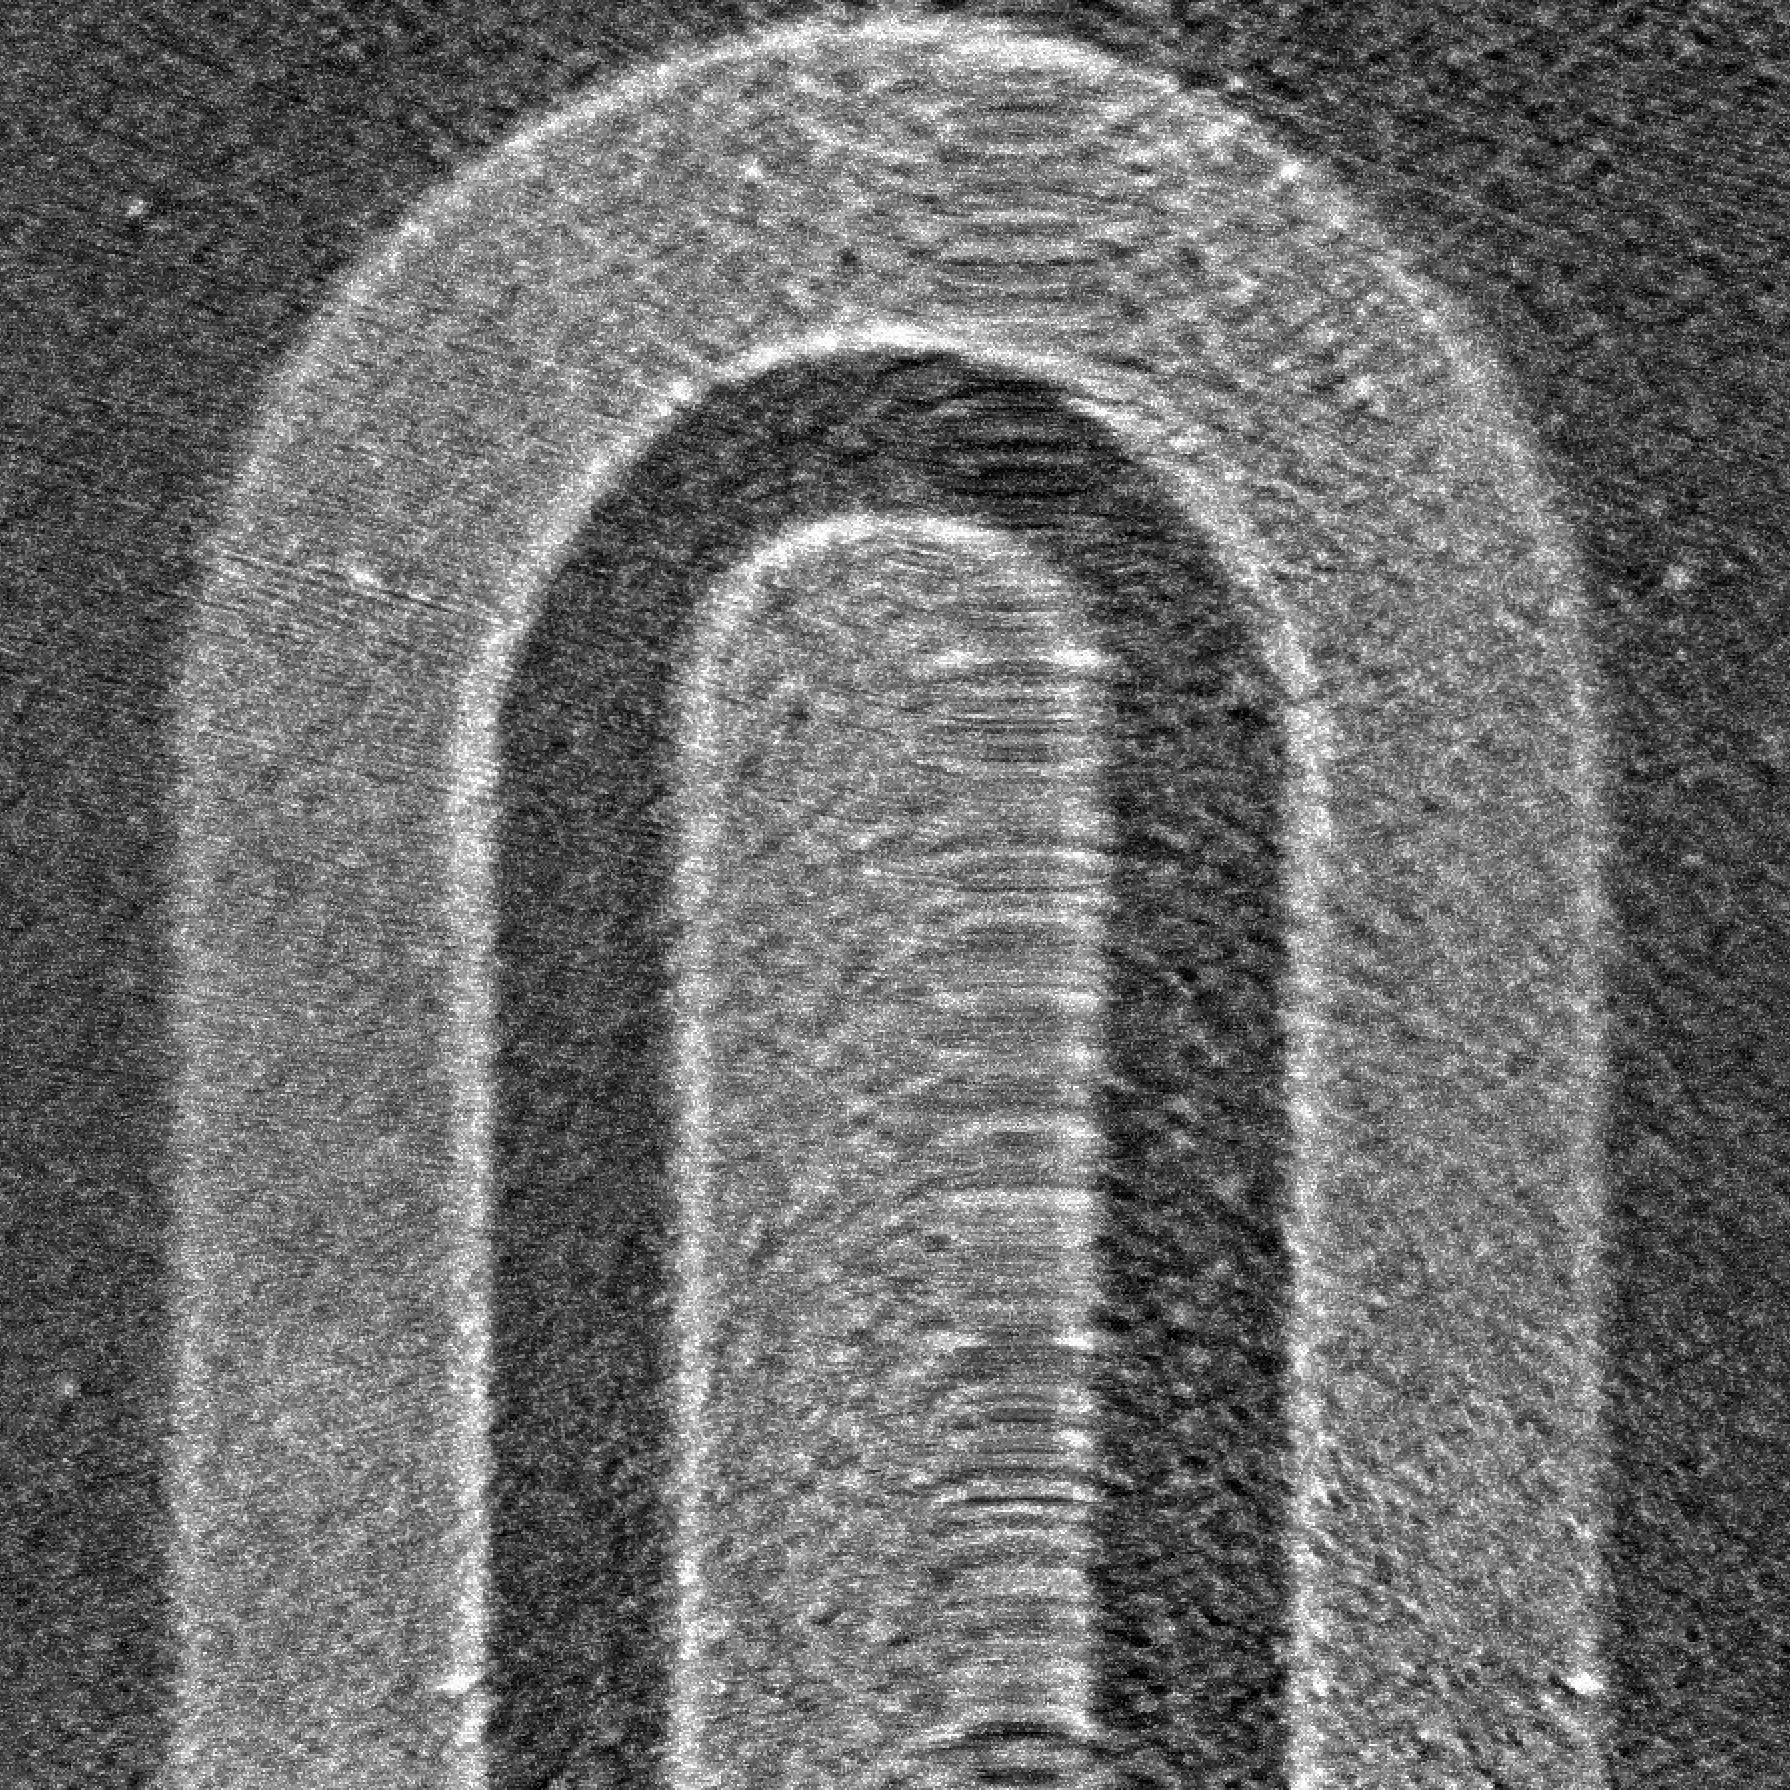
\includegraphics[width=0.9\linewidth]{Master Thesis Manuel Galdon/figures/Imaging/recon-filt-reslice-left.png}
\end{minipage}
\hfill
\begin{minipage}{0.53\textwidth}
    \centering
    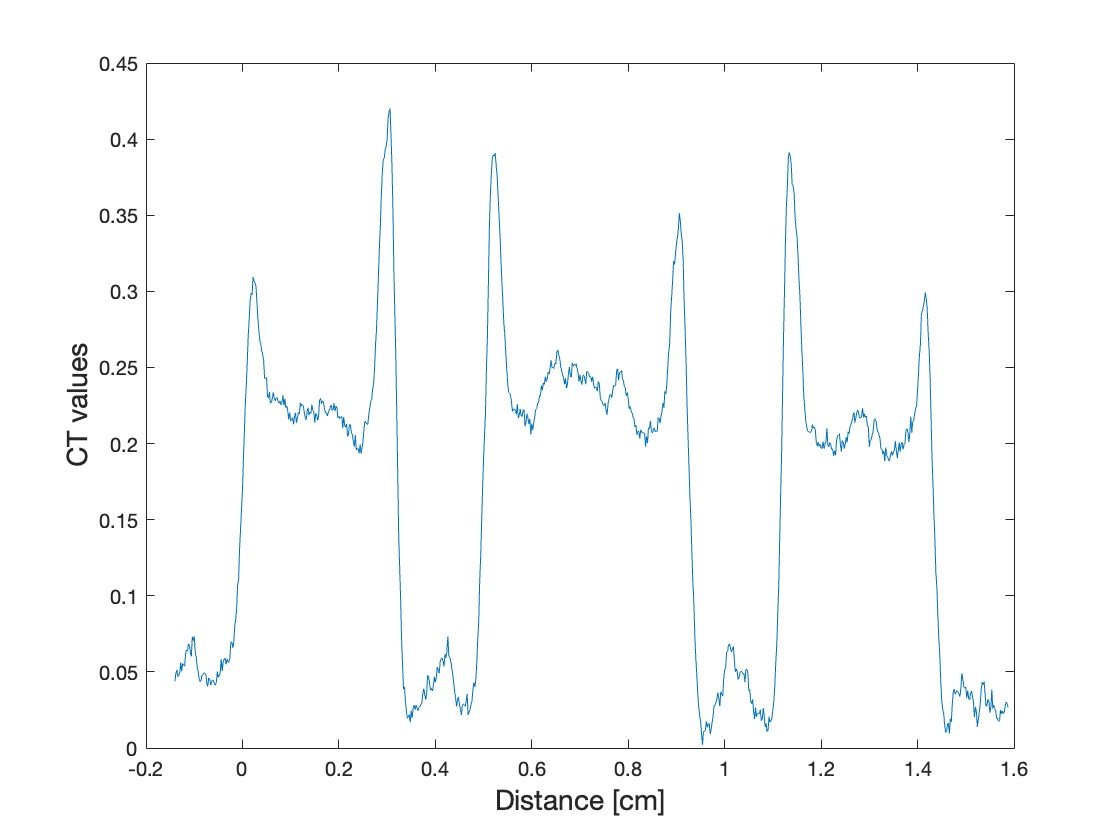
\includegraphics[width=1.1\linewidth]{Master Thesis Manuel Galdon/figures/Imaging/Neutron scan.jpg}
\end{minipage}
\caption{Neutron scan of TM33054 (left) and CT values vs. distance plot (right).}
\label{fig:Neutron scan vs plot}
\end{figure}

\newpage
The total thickness of the chamber is 1.4 \unit{\cm}, according to \textit{PTW Freiburg, Ionization chambers for neutron dosimetry} \cite{PTWKammerBauplan}. In the plot of Figure \ref{fig:Neutron scan vs plot}, the CT signal appears beyond the boundaries of the chamber. This is because the signal of the air around the chamber has also been plotted for statistical purposes. Even though the oxidation material is visible, it is not possible to identify its composition from neutron scan. However, the thickness can be \textbf{estimated}.

The CT values peak at the boundaries of the magnesium wall and the central anode with the surrounding environment. For each peak, the FWHM has been measured digitally. The full width half maximum provides the width of the CT value signal, which is, in the context of this neutron scan, the same as the layer.

The final result result has been averaged over all peaks. This average result is equal to:

\begin{align}
\label{eq:Averaged FWHM}
    0.37  	\pm 0.02 \; \unit{\milli\meter}
\end{align}

%It is interesting to note that the external corrosion layers i.e. the layer that are in contact with air are the thinnest with a thickness of 0.19 \si{\mm} both. In contrast, the inner layers, in contact with the argon gas, are averaged to 0.26 \si{\mm}. For the purpose of the MCNP simulations, the average thickness of 0.24 \si{\mm} has been used for all the layers. 